\documentclass[9.5pt, a4paper]{article}

% --- Essential Packages ---
\usepackage[utf8]{inputenc}
\usepackage[T1]{fontenc}
\usepackage{lmodern}
\usepackage[margin=0.5in, top=0.6in, bottom=0.55in]{geometry}
\usepackage[table,xcdraw]{xcolor}
\usepackage{listings}
\usepackage{tcolorbox}
\usepackage{enumitem}
\usepackage{hyperref}
\usepackage{fancyhdr}
\usepackage{titlesec}
\usepackage{graphicx}
\usepackage{booktabs}
\usepackage{amsmath}
\usepackage{amssymb}
\usepackage{tikz}
\usetikzlibrary{shapes.geometric, arrows.meta, positioning, calc, fit}
\usepackage{tabularx}
\usepackage{float}
\usepackage{caption}
\usepackage{parskip}
\usepackage{fontawesome5}

\tcbuselibrary{listings, skins, breakable}

% --- Color Palette ---
\definecolor{maindark}{HTML}{0f172a}       % Deep Slate
\definecolor{primary}{HTML}{4338ca}        % Indigo Accent
\definecolor{secondary}{HTML}{0369a1}      % Sky Blue Accent
\definecolor{accentgreen}{HTML}{047857}    % Emerald Accent
\definecolor{accentorange}{HTML}{b45309}   % Amber Accent
\definecolor{accentred}{HTML}{b91c1c}      % Crimson Accent
\definecolor{accentpurple}{HTML}{6d28d9}   % Violet Accent
\definecolor{codebg}{HTML}{1e293b}         % Dark code box
\definecolor{boxbg}{HTML}{f8fafc}          % Light slate bg
\definecolor{bordercol}{HTML}{cbd5e1}      % Border grey

% --- Hyperlink Setup ---
\hypersetup{
    colorlinks=true,
    linkcolor=primary,
    urlcolor=secondary,
    citecolor=accentgreen
}

% --- Code Listing Style ---
\lstdefinestyle{mystyle}{
    basicstyle=\ttfamily\scriptsize\color{white},
    backgroundcolor=\color{codebg},
    keywordstyle=\color{accentorange}\bfseries,
    stringstyle=\color{accentgreen},
    commentstyle=\color{bordercol}\itshape,
    numberstyle=\tiny\color{bordercol},
    numbers=none,
    frame=single,
    rulecolor=\color{primary},
    breaklines=true,
    tabsize=2,
    showstringspaces=false
}
\lstset{style=mystyle}

% --- tcolorbox Callout Boxes ---
\newtcolorbox{agentbox}[2][]{
    colback=boxbg, colframe=primary,
    fonttitle=\bfseries\footnotesize, title={\faIcon{robot} ~#2},
    boxrule=0.8pt, arc=3pt, top=3pt, bottom=3pt, left=4pt, right=4pt, #1
}
\newtcolorbox{conceptbox}[2][]{
    colback=boxbg, colframe=secondary,
    fonttitle=\bfseries\footnotesize, title={\faIcon{lightbulb} ~#2},
    boxrule=0.8pt, arc=3pt, top=3pt, bottom=3pt, left=4pt, right=4pt, #1
}
\newtcolorbox{interviewbox}[2][]{
    colback=boxbg, colframe=accentpurple,
    fonttitle=\bfseries\footnotesize, title={\faIcon{user-tie} ~#2},
    boxrule=1pt, arc=3pt, top=3pt, bottom=3pt, left=4pt, right=4pt, #1
}
\newtcolorbox{warningbox}[2][]{
    colback=boxbg, colframe=accentred,
    fonttitle=\bfseries\footnotesize, title={\faIcon{exclamation-triangle} ~#2},
    boxrule=0.8pt, arc=3pt, top=3pt, bottom=3pt, left=4pt, right=4pt, #1
}
\newtcolorbox{summarybox}[2][]{
    colback=boxbg, colframe=accentgreen,
    fonttitle=\bfseries\footnotesize, title={\faIcon{check-circle} ~#2},
    boxrule=0.8pt, arc=3pt, top=3pt, bottom=3pt, left=4pt, right=4pt, #1
}

% --- Page Header & Footer ---
\setlength{\headheight}{14pt}
\pagestyle{fancy}
\fancyhf{}
\fancyhead[L]{\textcolor{primary}{\textbf{\faIcon{project-diagram} Multi-Agent Research Orchestrator}} \footnotesize\textcolor{gray}{| 9-Page Master Revision Notes}}
\fancyhead[R]{\textcolor{accentpurple}{\footnotesize\textbf{GenAI Placement \& Interview Revision (Hinglish)}}}
\fancyfoot[L]{\textcolor{gray}{\scriptsize Autonomous Agentic Research Pipeline $\bullet$ LangGraph + Groq GPT-OSS-120B + ChromaDB + FastMCP}}
\fancyfoot[R]{\textcolor{primary}{\bfseries\small Page \thepage\ of 9}}
\renewcommand{\headrulewidth}{0.5pt}
\renewcommand{\footrulewidth}{0.4pt}

% --- Section Styling ---
\titleformat{\section}{\large\bfseries\color{primary}}{
    \colorbox{primary!10}{\makebox[1.6em]{\thesection}}}{0.3em}{}[
    \vspace{-0.4em}\color{primary}\rule{\textwidth}{1.2pt}]

\titleformat{\subsection}{\normalsize\bfseries\color{secondary}}{
    \thesubsection}{0.3em}{}[\vspace{-0.2em}\color{secondary!40}\rule{0.5\textwidth}{0.5pt}]

\setlist[itemize]{noitemsep, topsep=1pt, parsep=0pt, partopsep=0pt, leftmargin=12pt}
\setlist[enumerate]{noitemsep, topsep=1pt, parsep=0pt, partopsep=0pt, leftmargin=12pt}

\begin{document}

% ======================================================================
% PAGE 1: PROJECT OVERVIEW & CORE ARCHITECTURE
% ======================================================================
\begin{center}
    {\LARGE\bfseries\color{primary} \faIcon{microscope} Multi-Agent Research Orchestrator}\\[2pt]
    {\normalsize\bfseries\color{secondary} 9-Page Master Revision Notes \& Interview Preparation Blueprint (Hinglish)}\\[1pt]
    {\scriptsize\textbf{Core Tech Stack:} LangGraph StateGraph $\bullet$ Groq (GPT-OSS-120B) $\bullet$ ChromaDB Vector Store $\bullet$ FastMCP Protocol $\bullet$ Tavily Search $\bullet$ Streamlit UI}
\end{center}
\vspace{-6pt}
\hrule height 0.8pt
\vspace{4pt}

\section{Project Overview \& 4-Agent Architecture}

\begin{conceptbox}{Project Ka Core Problem \& Solution (Kyun Banaya?)}
Single LLM prompt ko jab bolte hain: \textit{``Research this topic and write a report''}, toh 3 badi problems aati hain:
1. \textbf{Hallucinations \& Fake Facts} (koi independent verification nahi hoti). 
2. \textbf{Superficial Summarization} (single-turn query saare angles cover nahi kar pati). 
3. \textbf{Zero Source Grounding} (unverified internet sources aur lack of internal document indexing).

\textbf{Our Engineering Solution:} Humne ek \textbf{Autonomous Multi-Agent State Machine} banaya using \textbf{LangGraph}. Yeh system \textbf{4 Specialized Agents} ko deploy karta hai jo ek real-world research firm ki tarah coordinate karte hain with an automated \textbf{Self-Correcting Revision Loop}, \textbf{Hybrid RAG (PDFs + Memory)}, aur \textbf{FastMCP Tool Server}.
\end{conceptbox}

\vspace{-4pt}
\subsection{System Architecture Diagram (LangGraph State Machine Pipeline)}
\vspace{-2pt}

\begin{center}
\begin{tikzpicture}[
    node distance=0.8cm and 1.3cm,
    agentnode/.style={draw=#1, rounded corners=5pt, fill=#1!8, text width=3.0cm,
                      align=center, minimum height=0.9cm, font=\scriptsize\bfseries, line width=1pt},
    routernode/.style={diamond, draw=accentred, fill=accentred!10, text width=1.8cm,
                       align=center, inner sep=1pt, font=\tiny\bfseries, line width=1pt},
    io/.style={draw=maindark, rounded corners=4pt, fill=maindark!5, text width=2.1cm,
               align=center, font=\tiny\bfseries},
    conn/.style={-{Stealth[length=2.2mm]}, line width=1.1pt, #1},
    lbl/.style={font=\tiny\bfseries, fill=white, inner sep=0.8pt}
]
    \node[io] (input) {User Query\\+ PDF Uploads};
    \node[agentnode=primary, right=0.9cm of input] (res) {\faIcon{search} Researcher Agent\\{\tiny (Tavily + Chroma RAG)}};
    \node[agentnode=secondary, right=0.9cm of res] (ana) {\faIcon{chart-bar} Analyst Agent\\{\tiny (Themes \& Discrepancies)}};
    \node[routernode, below=0.8cm of ana] (fc) {\faIcon{check-circle} Fact Checker\\{\tiny Evidence Verify}};
    \node[agentnode=accentgreen, left=0.9cm of fc] (wri) {\faIcon{pen-nib} Writer Agent\\{\tiny (Markdown + Memory)}};
    \node[io, left=0.9cm of wri] (output) {Verified Report\\+ ChromaDB Memory};

    \node[draw=accentorange, dashed, rounded corners=3pt, fill=accentorange!5, below=0.25cm of res, text width=2.8cm, align=center, font=\tiny\bfseries] (chroma) {
        \faIcon{database} ChromaDB Vector Store\\(all-MiniLM-L6-v2 Embeddings)
    };

    \draw[conn=primary] (input) -- (res) node[midway, above, lbl] {topic};
    \draw[conn=primary] (res) -- (ana) node[midway, above, lbl] {raw\_data};
    \draw[conn=secondary] (ana) -- (fc) node[midway, right, lbl] {analysis};
    \draw[conn=accentgreen] (fc) -- (wri) node[midway, above, lbl] {PASSED};
    \draw[conn=accentgreen] (wri) -- (output) node[midway, above, lbl] {report};

    % Self-correction feedback loop
    \draw[conn=accentred, dashed] (fc.west) -| node[near start, below, lbl] {NEEDS\_REVISION (Max 2)} (res.south);
    \draw[conn=accentorange, dotted] (res.south) -- (chroma.north);
    \draw[conn=accentorange, dotted] (wri.south) |- (chroma.east);
\end{tikzpicture}
\end{center}

\vspace{-6pt}
\subsection{The 4 Specialized Agents Role Matrix}
\vspace{-2pt}

\begin{table}[H]
\centering
\scriptsize
\begin{tabularx}{\textwidth}{l p{2.4cm} p{5.5cm} X}
\toprule
\rowcolor{primary!10}
\textbf{Agent Name} & \textbf{Core Role} & \textbf{Tools \& Operations Executed} & \textbf{Prompting Strategy \& Temp} \\
\midrule
\textbf{1. Researcher} & Multi-angle Search \& RAG & Query expansion (3 sub-queries), Tavily Web API, ChromaDB vector retrieval for uploaded PDFs. & $T=0.0$ (Strict factual retrieval without hallucination). \\
\textbf{2. Analyst} & Intelligence Synthesis & Aggregates findings into themes, highlights consensus, identifies source contradictions and missing gaps. & $T=0.1$ (Structured synthesis, JSON-like categorization). \\
\textbf{3. Fact-Checker} & Evidence Verification & Cross-verifies claims against raw retrieved evidence. Emits verdict: \texttt{PASSED} or \texttt{NEEDS\_REVISION}. & $T=0.0$ (Adversarial closed-world source grounding). \\
\textbf{4. Writer} & Publication \& Memory & Synthesizes verified analysis into structured Markdown with citations, saves session to ChromaDB memory. & $T=0.3$ (Executive formatting, high prose clarity). \\
\bottomrule
\end{tabularx}
\end{table}

\vspace{-4pt}
\begin{summarybox}{3 Key Highlights Jo Interview Mein Bolne Hain}
1. \textbf{Stateful Loop Control:} LangGraph StateGraph se bounded feedback loop implement kiya hai jo unverified claims ko automatically fix karta hai.\\
2. \textbf{Zero Cost / High Speed:} Groq LPUs par GPT-OSS-120B running at 250+ tok/s + Local MiniLM embeddings = Zero API cost.\\
3. \textbf{Universal MCP Compatibility:} FastMCP server expose karta hai research engine tools for Claude Desktop and Cursor.
\end{summarybox}

\clearpage
% ======================================================================
% PAGE 2: LANGGRAPH STATE SCHEMA & STATE MACHINE
% ======================================================================
\section{LangGraph State Schema \& State Machine Workflow}

\begin{conceptbox}{LangGraph State Management Pattern (TypedDict with Reducers)}
LangGraph mein agents ek dusre ko direct parameter nahi bhejte. Ek central \textbf{State Dictionary} hoti hai. Jab koi agent apna kaam karta hai, wo state ko update karta hai. LangGraph ka \textbf{Reducer Pattern} ensure karta hai ki dynamic loops ke dauran purana context overwrite na ho.
\end{conceptbox}

\vspace{-4pt}
\subsection{1. Central State Schema Definition (\texttt{state/schema.py})}

\begin{lstlisting}[language=Python]
from typing import TypedDict, Annotated, List, Optional
import operator

class ResearchState(TypedDict):
    topic: str                                         # User ka initial research query
    uploaded_docs: Optional[List[str]]                 # User ke upload kiye huye PDF files
    research_data: Annotated[List[str], operator.add]  # Append-only reducer for search results
    analysis: Optional[str]                            # Analyst agent ka structured output
    fact_check_feedback: Optional[str]                 # Fact checker ke feedback notes
    revision_count: int                                # Infinite loop prevention counter (Max 2)
    final_report: Optional[str]                        # Final generated markdown report
    logs: Annotated[List[str], operator.add]           # Real-time UI streaming logs
\end{lstlisting}

\begin{conceptbox}{Reducer Concept: \texttt{Annotated[List[str], operator.add]} Kaise Kaam Karta Hai?}
\begin{itemize}
    \item \textbf{Normal Dict behavior:} Agar \texttt{research\_data} ek plain list hoti, toh loop ke second iteration par naya search data purane search data ko \textbf{overwrite} kar deta.
    \item \textbf{Reducer magic:} \texttt{operator.add} LangGraph ko instruct karta hai: \textit{``Jab bhi koi node naya list chunk return kare, use existing list ke end mein concatenate (+) karo.''}
\end{itemize}
\end{conceptbox}

\vspace{-4pt}
\subsection{2. State Graph Assembly \& Conditional Routing (\texttt{graph/workflow.py})}

\begin{lstlisting}[language=Python]
from langgraph.graph import StateGraph, END
from state.schema import ResearchState
from agents.researcher import researcher_node
from agents.analyst import analyst_node
from agents.fact_checker import fact_checker_node
from agents.writer import writer_node

def should_continue(state: ResearchState) -> str:
    """Conditional Edge: Decides whether to loop back or proceed to writing."""
    feedback = state.get("fact_check_feedback", "")
    rev_count = state.get("revision_count", 0)
    
    # Self-Correction Guardrail: Max 2 revisions allowed
    if "NEEDS_REVISION" in feedback and rev_count < 2:
        return "researcher"  # Feedback loop
    return "writer"          # Passed or Max revisions reached

def build_graph():
    workflow = StateGraph(ResearchState)
    
    # 1. Register all Agent Nodes
    workflow.add_node("researcher", researcher_node)
    workflow.add_node("analyst", analyst_node)
    workflow.add_node("fact_checker", fact_checker_node)
    workflow.add_node("writer", writer_node)

    # 2. Linear Edges
    workflow.set_entry_point("researcher")
    workflow.add_edge("researcher", "analyst")
    workflow.add_edge("analyst", "fact_checker")

    # 3. Dynamic Routing Edge
    workflow.add_conditional_edges(
        "fact_checker",
        should_continue,
        {"researcher": "researcher", "writer": "writer"}
    )
    workflow.add_edge("writer", END)
    return workflow.compile()
\end{lstlisting}

\begin{summarybox}{State Machine Ke 3 Safety Guarantees}
1. \textbf{Deterministic Execution:} Pipeline always starts at \texttt{researcher} and cleanly finishes at \texttt{writer} $\rightarrow$ \texttt{END}.\\
2. \textbf{Loop Guardrail:} Bounded counter (\texttt{rev\_count < 2}) prevents infinite token burn and API deadlocks.\\
3. \textbf{State Isolation:} Har node sirf wohi keys modify karta hai jinke liye wo authorized hai.
\end{summarybox}

\clearpage
% ======================================================================
% PAGE 3: THE 4 AGENTS IN-DEPTH DEEP DIVE
% ======================================================================
\section{The 4 Agents In-Depth: Prompts, Logic \& Execution}

\subsection{1. Researcher Agent (\texttt{agents/researcher.py})}
\begin{agentbox}{Researcher Logic: Multi-Query Search + Local Vector RAG}
\begin{itemize}
    \item \textbf{Query Expansion:} LLM ko prompt karke topic ke 3 specific sub-queries generate karwata hai (e.g., 1. Market overview, 2. Technical breakthroughs, 3. Critical challenges).
    \item \textbf{Dual Retrieval Execution:}
    \begin{itemize}
        \item \textbf{Tavily Web API:} Top 5 verified live web pages fetch karta hai.
        \item \textbf{ChromaDB Vector Store:} Uploaded PDFs se semantic similarity search karke top 4 context chunks retrieve karta hai.
    \end{itemize}
    \item \textbf{Feedback-Driven Search:} Agar state mein \texttt{fact\_check\_feedback} hai, toh un missing claims ke liye targeted queries run karta hai.
\end{itemize}
\end{agentbox}

\vspace{-4pt}
\subsection{2. Analyst Agent (\texttt{agents/analyst.py})}
\begin{agentbox}{Analyst Logic: Raw Data to Thematic Intelligence}
Raw search data chaotic aur redundant hota hai. Analyst agent raw text ko structured framework mein convert karta hai:
\begin{enumerate}
    \item \textbf{Core Thematic Synthesis:} Primary concepts ko categorized bullet points mein break karna.
    \item \textbf{Consensus Points:} Multiple sources kin key findings par agree karte hain.
    \item \textbf{Contradictions / Discrepancies:} Agar Source A aur Source B mein numerical ya timeline conflict hai, usko explicitly flag karna.
    \item \textbf{Knowledge Gaps:} Konsi critical details abhi bhi unverified hain.
\end{enumerate}
\end{agentbox}

\vspace{-4pt}
\subsection{3. Fact-Checker Agent (\texttt{agents/fact\_checker.py})}
\begin{agentbox}{Fact-Checker Logic: Adversarial Source Grounding}
\begin{itemize}
    \item \textbf{Strict Closed-World Check:} Analyst ke har key claim ko raw \texttt{research\_data} ke saath compare karta hai.
    \item \textbf{Decision Output:}
    \begin{itemize}
        \item \texttt{PASSED}: Claims are directly supported by evidence $\rightarrow$ Proceed to Writer.
        \item \texttt{NEEDS\_REVISION}: Unsupported claim detected $\rightarrow$ Return specific missing evidence notes and increment \texttt{revision\_count}.
    \end{itemize}
\end{itemize}
\end{agentbox}

\vspace{-4pt}
\subsection{4. Writer Agent (\texttt{agents/writer.py})}
\begin{agentbox}{Writer Logic: Publication Synthesis \& Memory Persistence}
\begin{itemize}
    \item \textbf{Markdown Formatting:} Title, Executive Summary, Deep Findings, Contradictions, Strategic Recommendations, Citations.
    \item \textbf{Long-Term Vector Memory:} Report generate hote hi \texttt{store\_research\_session()} call karke ChromaDB collection \texttt{"research\_memory"} mein session embedding save kar deta hai.
\end{itemize}
\end{agentbox}

\vspace{-4pt}
\subsection{Temperature \& Tuning Strategy}
\begin{table}[H]
\centering
\scriptsize
\begin{tabularx}{\textwidth}{l c l X}
\toprule
\rowcolor{primary!10}
\textbf{Agent} & \textbf{Temperature} & \textbf{Why this exact setting?} & \textbf{Risk if setting is wrong} \\
\midrule
\textbf{Researcher} & \textbf{0.0} & Zero creativity; pure deterministic query extraction. & High temp causes hallucinated keywords. \\
\textbf{Analyst} & \textbf{0.1} & Strict logical deduction and thematic grouping. & High temp creates loose, invalid relations. \\
\textbf{Fact-Checker} & \textbf{0.0} & Zero tolerance for assumptions; adversarial verification. & High temp misses unverified claims. \\
\textbf{Writer} & \textbf{0.3} & Smooth readability, professional executive prose. & Zero temp makes writing stiff and robotic. \\
\bottomrule
\end{tabularx}
\end{table}

\clearpage
% ======================================================================
% PAGE 4: RAG SYSTEM & VECTOR DATABASE ARCHITECTURE
% ======================================================================
\section{RAG System \& Dual-Purpose Vector Memory}

\begin{conceptbox}{Dual-Purpose Knowledge Architecture}
Is system mein RAG sirf ek simple PDF reader nahi hai — yeh \textbf{2 Distinct Lifecycles} manage karta hai:
1. \textbf{Short-Term Document Ingestion:} User dwara upload kiye gaye dynamic PDF research papers ko chunk karke instant query context provide karna.
2. \textbf{Long-Term Episodic Memory:} Har research session ki key findings ko ChromaDB mein store karna taaki future sessions past research ko leverage kar sakein.
\end{conceptbox}

\vspace{-4pt}
\subsection{RAG Pipeline Flowchart}

\begin{center}
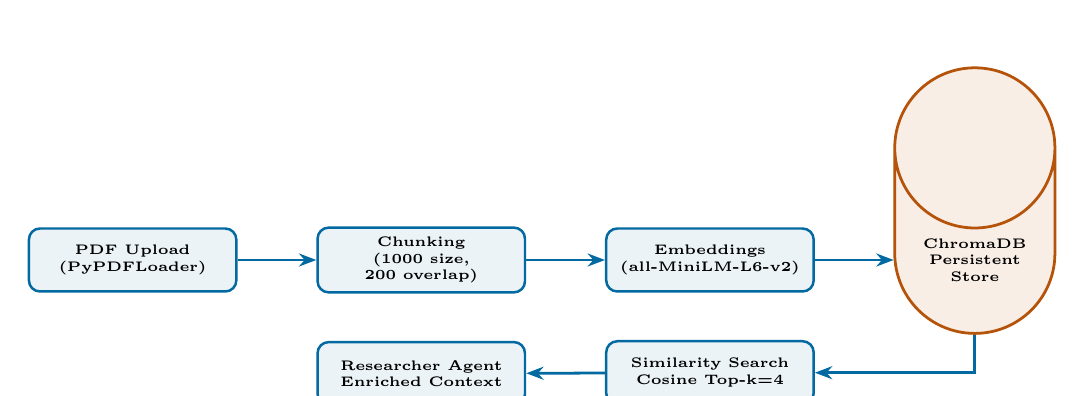
\begin{tikzpicture}[
    node distance=0.6cm and 1.0cm,
    stepnode/.style={draw=secondary, rounded corners=4pt, fill=secondary!8, text width=2.4cm,
                     align=center, minimum height=0.8cm, font=\tiny\bfseries, line width=0.9pt},
    storenode/.style={cylinder, shape border rotate=90, draw=accentorange, fill=accentorange!10,
                      text width=1.8cm, align=center, font=\tiny\bfseries, minimum height=1.0cm, line width=1pt},
    conn/.style={-{Stealth[length=2.2mm]}, line width=1pt, secondary}
]
    \node[stepnode] (doc) {PDF Upload\\{\tiny (PyPDFLoader)}};
    \node[stepnode, right=of doc] (split) {Chunking\\{\tiny (1000 size, 200 overlap)}};
    \node[stepnode, right=of split] (embed) {Embeddings\\{\tiny (all-MiniLM-L6-v2)}};
    \node[storenode, right=of embed] (chroma) {ChromaDB\\{\tiny Persistent Store}};
    \node[stepnode, below=0.6cm of embed] (query) {Similarity Search\\{\tiny Cosine Top-k=4}};
    \node[stepnode, below=0.6cm of split] (agent) {Researcher Agent\\{\tiny Enriched Context}};

    \draw[conn] (doc) -- (split);
    \draw[conn] (split) -- (embed);
    \draw[conn] (embed) -- (chroma);
    \draw[conn] (chroma) |- (query);
    \draw[conn] (query) -- (agent);
\end{tikzpicture}
\end{center}

\vspace{-4pt}
\subsection{RAG Code Implementation Details (\texttt{rag/vector\_store.py})}

\begin{lstlisting}[language=Python]
from langchain_community.document_loaders import PyPDFLoader
from langchain_text_splitters import RecursiveCharacterTextSplitter
from langchain_huggingface import HuggingFaceEmbeddings
from langchain_community.vectorstores import Chroma
from config.settings import settings

def get_embeddings():
    # Local 384-dimensional dense embeddings (Zero API cost, fast CPU inference)
    return HuggingFaceEmbeddings(model_name="sentence-transformers/all-MiniLM-L6-v2")

def ingest_pdf(file_path: str) -> int:
    loader = PyPDFLoader(file_path)
    docs = loader.load()
    
    # Recursive splitting preserves paragraphs and sentences
    splitter = RecursiveCharacterTextSplitter(chunk_size=1000, chunk_overlap=200)
    chunks = splitter.split_documents(docs)
    
    vectorstore = Chroma(
        collection_name="research_docs",
        embedding_function=get_embeddings(),
        persist_directory=settings.CHROMA_PERSIST_DIR
    )
    vectorstore.add_documents(chunks)
    return len(chunks)

def retrieve_context(query: str, k: int = 4) -> str:
    vectorstore = Chroma(
        collection_name="research_docs",
        embedding_function=get_embeddings(),
        persist_directory=settings.CHROMA_PERSIST_DIR
    )
    results = vectorstore.similarity_search(query, k=k)
    return "\n\n".join([doc.page_content for doc in results])
\end{lstlisting}

\vspace{-4pt}
\subsection{RAG Technical Justifications (Interview Gold)}
\begin{summarybox}{RAG Design Choices: Why This Setup?}
\begin{itemize}
    \item \textbf{Why \texttt{RecursiveCharacterTextSplitter}?} Normal splitters arbitrary length par split karte hain jisse words ya code toot jata hai. Recursive splitter pehle double newlines (\texttt{\textbackslash n\textbackslash n}), fir single newlines (\texttt{\textbackslash n}), fir spaces par split karta hai — ensuring semantic paragraph integrity.
    \item \textbf{Why Chunk Size = 1000 \& Overlap = 200?} 1000 characters ($\sim$200 words) ek complete concept capture karta hai. 200 characters overlap ensure karta hai ki chunk boundary par key context lost na ho.
    \item \textbf{Why \texttt{all-MiniLM-L6-v2} Embeddings?} Light-weight (80MB), runs locally on CPU with zero latency and zero API cost, generating high-quality 384-dimensional embeddings.
\end{itemize}
\end{summarybox}

\clearpage
% ======================================================================
% PAGE 5: FAST-MCP PROTOCOL & STREAMLIT UI
% ======================================================================
\section{Model Context Protocol (MCP) Server \& Streamlit UI}

\begin{conceptbox}{MCP (Model Context Protocol) Architecture}
Anthropic ka \textbf{Model Context Protocol (MCP)} ek open universal standard hai jo AI assistants (jaise Claude Desktop, Cursor IDE) ko external tools aur data stores se connect karta hai. Humne pure research pipeline ko ek \textbf{FastMCP Server} ke roop mein expose kiya hai.
\end{conceptbox}

\vspace{-4pt}
\subsection{FastMCP Architecture \& Exposed Tools}

\begin{center}
\begin{tikzpicture}[
    node distance=0.8cm and 1.4cm,
    clientnode/.style={draw=accentpurple, rounded corners=5pt, fill=accentpurple!8, text width=2.4cm,
                       align=center, minimum height=0.9cm, font=\tiny\bfseries, line width=1pt},
    mcpbox/.style={draw=primary, rounded corners=6pt, fill=primary!5, text width=4.2cm,
                   align=center, minimum height=2.0cm, font=\scriptsize\bfseries, line width=1.1pt},
    toolnode/.style={draw=accentgreen, rounded corners=3pt, fill=accentgreen!10, text width=3.6cm,
                     align=left, font=\tiny\ttfamily, inner sep=2pt},
    conn/.style={-{Stealth[length=2.4mm]}, line width=1.1pt}
]
    \node[clientnode] (claude) {\faIcon{desktop} Claude Desktop\\{\tiny (via Stdio)}};
    \node[clientnode, below=0.6cm of claude] (cursor) {\faIcon{terminal} Cursor IDE\\{\tiny (via Stdio / SSE)}};
    
    \node[mcpbox, right=of claude, yshift=-0.4cm] (mcp) {
        \textbf{\faIcon{plug} FastMCP Server (\texttt{mcp\_server.py})}\\[2pt]
        \begin{tikzpicture}
            \node[toolnode] (t1) {@mcp.tool() research\_topic()};
            \node[toolnode, below=2pt of t1] (t2) {@mcp.tool() ingest\_document()};
            \node[toolnode, below=2pt of t2] (t3) {@mcp.tool() search\_knowledge\_base()};
        \end{tikzpicture}
    };
    
    \node[clientnode, right=of mcp] (graph) {\faIcon{project-diagram} LangGraph\\Research Graph};

    \draw[conn, accentpurple] (claude) -- (mcp.west |- claude);
    \draw[conn, accentpurple] (cursor) -- (mcp.west |- cursor);
    \draw[conn, primary] (mcp) -- (graph);
\end{tikzpicture}
\end{center}

\vspace{-4pt}
\subsection{FastMCP Server Code (\texttt{mcp\_server.py})}

\begin{lstlisting}[language=Python]
from fastmcp import FastMCP
from graph.workflow import build_graph
from rag.vector_store import ingest_pdf, retrieve_context

mcp = FastMCP("Multi-Agent-Research-Orchestrator")

@mcp.tool()
def research_topic(topic: str) -> str:
    """Executes the full 4-agent LangGraph workflow and returns verified markdown report."""
    graph = build_graph()
    initial_state = {"topic": topic, "research_data": [], "revision_count": 0, "logs": []}
    result = graph.invoke(initial_state)
    return result.get("final_report", "Research pipeline failed.")

@mcp.tool()
def ingest_document(pdf_path: str) -> str:
    """Ingests local PDF into ChromaDB vector memory for future research."""
    num_chunks = ingest_pdf(pdf_path)
    return f"Successfully ingested {num_chunks} chunks from {pdf_path}"

if __name__ == "__main__":
    mcp.run(transport="stdio")
\end{lstlisting}

\vspace{-4pt}
\subsection{Streamlit UI Capabilities (\texttt{app.py})}
\begin{summarybox}{Streamlit Frontend Highlights}
\begin{itemize}
    \item \textbf{Real-Time Agent Stepping Logs:} LangGraph execution stream ko consume karke real-time dynamic spinner aur activity logs display karta hai.
    \item \textbf{Glassmorphism Dark Theme:} CSS injection se custom modern interface with 3 themes: \textit{Emerald Slate, Dark Slate, Clean Light}.
    \item \textbf{Document Upload \& Downloads:} Direct PDF drag-and-drop ingestion, along with instant \texttt{.md} and \texttt{.txt} report downloads.
\end{itemize}
\end{summarybox}

\clearpage
% ======================================================================
% PAGE 6: END-TO-END EXECUTION FLOW & CONFIGURATION
% ======================================================================
\section{End-to-End Execution Flow \& Production Configuration}

\subsection{1. Step-by-Step Execution Lifecycle Walkthrough}

\begin{enumerate}
    \item \textbf{Session Kickoff:} User inputs query: \textit{``Next-Gen Solid State Battery Market 2026''} and uploads an OEM technical paper.
    \item \textbf{Researcher Agent:}
    \begin{itemize}
        \item Expands into 3 sub-queries: (a) Commercial timelines, (b) Energy density comparisons, (c) Manufacturing bottleneck yield rates.
        \item Calls Tavily Web Search $\rightarrow$ Fetches 5 live web pages.
        \item Calls ChromaDB Similarity Search $\rightarrow$ Fetches 4 top chunks from uploaded OEM paper.
    \end{itemize}
    \item \textbf{Analyst Agent:} Synthesizes raw findings into: \textit{Key Themes (Solid electrolytes), Consensus (Higher safety), Contradiction (Toyota 2027 vs QuantumScape 2025 timeline), Knowledge Gap (Yield rate at mass scale)}.
    \item \textbf{Fact-Checker Agent (First Pass):}
    \begin{itemize}
        \item Checks statement: \textit{``QuantumScape achieved 99.8\% commercial yield in 2025''}.
        \item Cross-checks raw \texttt{research\_data} $\rightarrow$ Source only claims pilot line testing, not 99.8\% commercial yield!
        \item \textbf{Triggers Revision:} Returns verdict \texttt{NEEDS\_REVISION: Verify commercial yield rate claims}.
        \item Increments \texttt{revision\_count = 1} $\rightarrow$ Conditional router sends state back to \textbf{Researcher}.
    \end{itemize}
    \item \textbf{Targeted Re-Research:} Researcher executes focused search on \textit{``QuantumScape verified pilot separator yield reports''} and appends clean evidence.
    \item \textbf{Re-Analysis \& Approval:} Analyst refines brief $\rightarrow$ Fact Checker validates and returns \texttt{PASSED}.
    \item \textbf{Writer Agent \& Persistence:} Formats comprehensive Markdown report with inline citations $\rightarrow$ Stores session embeddings into ChromaDB memory $\rightarrow$ Streams report to Streamlit UI.
\end{enumerate}

\vspace{-4pt}
\subsection{2. Production Configuration (\texttt{config/setting.py})}

\begin{lstlisting}[language=Python]
from pydantic_settings import BaseSettings

class Settings(BaseSettings):
    # LLM Inference
    GROQ_API_KEY: str
    MODEL_NAME: str = "openai/gpt-oss-120b"
    
    # Search Engine
    TAVILY_API_KEY: str
    MAX_SEARCH_RESULTS: int = 5
    
    # Guardrails
    MAX_REVISIONS: int = 2
    
    # Vector Database
    CHROMA_PERSIST_DIR: str = "./chroma_db"
    EMBEDDING_MODEL: str = "sentence-transformers/all-MiniLM-L6-v2"
    CHUNK_SIZE: int = 1000
    CHUNK_OVERLAP: int = 200

    class Config:
        env_file = ".env"

settings = Settings()
\end{lstlisting}

\begin{warningbox}{Production Security \& Graceful Fallback}
\begin{itemize}
    \item API keys are loaded strictly through \texttt{pydantic-settings} with type validation.
    \item Agar Tavily API rate limit hit hoti hai, system silently ChromaDB local documents par fallback karta hai without crashing.
\end{itemize}
\end{warningbox}

\clearpage
% ======================================================================
% PAGE 7 (INTERVIEW PART 1): WHY CHOOSE MATRIX & ARCHITECTURAL DECISIONS
% ======================================================================
\section{Interview Deep-Dive Part 1: The ``Why Choose'' Decision Matrix}

\begin{conceptbox}{What Interviewers Evaluate Here}
Interviewer yeh dekhna chahta hai ki aapne technologies blindly select ki hain ya \textbf{Engineering Trade-offs} samajh kar select ki hain.
\end{conceptbox}

\subsection{Key Architectural Justifications \& Comparisons}

\begin{interviewbox}{Q1: LangGraph kyun choose kiya? CrewAI ya AutoGen kyun nahi use kiya?}
\textbf{Hinglish Answer:}
\begin{itemize}
    \item \textbf{LangGraph vs CrewAI:} CrewAI role-playing agents ke liye beginner-friendly hai, lekin wo ek \textbf{black-box} framework hai jisme state flow aur cyclic routing par fine-grained programmatic control nahi milta. LangGraph explicit \textbf{State Machine (DAG with cycles)} provide karta hai jisme conditional edges, explicit reducers, aur cyclic feedback loops cleanly implement hote hain.
    \item \textbf{LangGraph vs AutoGen:} AutoGen conversational chat pattern use karta hai (agents ek dusre se continuous chat karte hain), jisme infinite chat loops, high latency aur massive token burn ka risk hota hai. LangGraph ek structured schema (\texttt{TypedDict}) ke through deterministic state pass karta hai, jo enterprise applications ke liye reliable aur predictable hai.
\end{itemize}
\end{interviewbox}

\begin{interviewbox}{Q2: 4 alag agents kyun banaye? Ek hi LLM call mein sab kyun nahi karwaya?}
\textbf{Hinglish Answer:}
\begin{enumerate}
    \item \textbf{Separation of Concerns:} Ek single prompt ko bolna ki \textit{``Search karo, analyze karo, fact-check karo, aur report likho''} results in mediocre output at every single step.
    \item \textbf{Role-Specific Temperature Tuning:} Researcher ($T=0.0$, strictly factual), Analyst ($T=0.1$, structured reasoning), Fact-Checker ($T=0.0$, adversarial verification), Writer ($T=0.3$, fluent prose). Single prompt mein multiple temperatures impossible hain.
    \item \textbf{Confirmation Bias Mitigation:} LLM apne hi generated text ki mistakes ko easily identify nahi kar pata. Fact-Checker ko as an independent adversary run karne se hallucinations catch ho jati hain.
    \item \textbf{Modularity:} Future mein naye agents (e.g., Data Visualizer, Code Sandbox) add karna bina existing graph ko tode aasan hai.
\end{enumerate}
\end{interviewbox}

\begin{interviewbox}{Q3: Groq LPU + GPT-OSS-120B kyun use kiya? OpenAI GPT-4o kyun nahi?}
\textbf{Hinglish Answer:}
\begin{itemize}
    \item \textbf{Inference Speed (LPUs):} Multi-agent pipeline mein 4--6 sequential LLM calls hoti hain. GPT-4o par yeh pipeline 30--45 seconds leti, jabki Groq LPUs par 250+ tokens/sec ki speed se yeh \textbf{6--8 seconds} mein complete ho jata hai.
    \item \textbf{Zero API Cost:} Groq free/low-cost tiers + local MiniLM embeddings = Zero infrastructure bill for deployment.
    \item \textbf{Reasoning Quality:} GPT-OSS-120B structured JSON generation aur analytical reasoning mein GPT-4 class models ke barabar compete karta hai.
\end{itemize}
\end{interviewbox}

\begin{interviewbox}{Q4: State schema ke liye TypedDict kyun choose kiya? Pydantic BaseModel kyun nahi?}
\textbf{Hinglish Answer:}
\begin{itemize}
    \item \textbf{Performance:} \texttt{TypedDict} runtime par pure standard Python dict hai, jisme zero schema validation latency hoti hai during high-frequency agent state transitions.
    \item \textbf{Reducer Integration:} LangGraph ka \texttt{Annotated[list, operator.add]} reducer pattern TypedDict ke sath seamlessly support hota hai. Pydantic use karte toh extra custom root validators likhne padte.
\end{itemize}
\end{interviewbox}

\clearpage
% ======================================================================
% PAGE 8 (INTERVIEW PART 2): CHALLENGES & ENGINEERING SOLUTIONS
% ======================================================================
\section{Interview Deep-Dive Part 2: Top 5 Real-World Engineering Challenges}

\begin{conceptbox}{What Interviewers Look For}
Senior AI Engineer interviews mein sabse deciding question hota hai: \textit{``What were the biggest technical blockers you faced while building this multi-agent system, and how did you resolve them?''}
\end{conceptbox}

\subsection{5 Real-World Production Challenges Solved in this Project}

\begin{interviewbox}{Challenge 1: Preventing Infinite Revision Loops \& Token Drain}
\textbf{Problem:} Agar Fact-Checker ko har pass par koi minor discrepancy milti rahe, toh graph infinite loop \texttt{Researcher $\leftrightarrow$ Fact-Checker} mein phas sakta tha, leading to API rate-limit crashes aur token waste.\\
\textbf{My Solution:} 
\begin{itemize}
    \item State schema mein \texttt{revision\_count: int} guardrail counter implement kiya.
    \item Router function \texttt{should\_continue()} strict bound enforce karta hai:
    \texttt{if "NEEDS\_REVISION" in feedback and rev\_count < 2: return "researcher" else: return "writer"}.
    \item Max limit (2) reach hone par pipeline crash hone ke bajaye Writer ko \textit{``Unverified Discrepancy Note''} forward karta hai, jo report ke Limitations section mein publish ho jata hai.
\end{itemize}
\end{interviewbox}

\begin{interviewbox}{Challenge 2: LLM Self-Confirmation Bias in Fact-Checking}
\textbf{Problem:} Fact-Checker agent aksar apne internal pre-training weights se assumptions bana leta tha bajaye raw retrieved evidence ko strictly check karne ke.\\
\textbf{My Solution:}
\begin{itemize}
    \item \textbf{Closed-World Assumption Prompting:} Prompt mein explicitly likha: \textit{``You are a strict legal auditor. ONLY verify a claim if direct verbatim evidence exists in `research\_data`. Outside general knowledge is considered INVALID.''}
    \item Temperature ko strictly \textbf{0.0} par lock kiya and required structured output with evidence quotes.
\end{itemize}
\end{interviewbox}

\begin{interviewbox}{Challenge 3: Context Window Bloat \& Latency Explosion}
\textbf{Problem:} Multi-query Tavily searches aur PDF documents se raw context 50KB+ ho jata tha, jo downstream Writer agent ke context window aur token cost ko explode kar raha tha.\\
\textbf{My Solution:}
\begin{itemize}
    \item Analyst agent ko ek \textbf{Lossless Context Condenser} ki tarah design kiya.
    \item Writer agent ko pure 50KB raw search dumps bhejne ke bajaye Analyst ka 2KB highly dense, structured intelligence brief pass kiya — reducing Writer token consumption by 85\%.
\end{itemize}
\end{interviewbox}

\begin{interviewbox}{Challenge 4: Handling Contradictory Information (Web vs Uploaded PDFs)}
\textbf{Problem:} Uploaded corporate whitepaper (e.g., 2023) aur live web data (2026) aapas mein contradict karte the.\\
\textbf{My Solution:}
\begin{itemize}
    \item Chunk metadata mein source tagging lagayi: \texttt{\{"source\_type": "uploaded\_doc"\}} vs \texttt{\{"source\_type": "live\_web"\}}.
    \item Analyst agent mein explicit \textbf{Contradictions Section} create kiya jo dono perspectives ko neutrally juxtapose karta hai.
\end{itemize}
\end{interviewbox}

\begin{interviewbox}{Challenge 5: Network API Failures \& Graceful Degradation}
\textbf{Problem:} Agar Tavily web search API network timeout de ya ChromaDB corrupt ho jaye, toh entire graph crash ho jata tha.\\
\textbf{My Solution:}
\begin{itemize}
    \item Robust \texttt{try-except} handlers lagaye. Agar Tavily search fail hoti hai, pipeline gracefully ChromaDB local vector store se available context use karke aage badhti hai with a clear warning log.
\end{itemize}
\end{interviewbox}

\clearpage
% ======================================================================
% PAGE 9 (INTERVIEW PART 3): TOUGH QUESTIONS & PRODUCTION SCALING
% ======================================================================
\section{Interview Deep-Dive Part 3: Tough Technical Q\&A \& Production Scaling}

\subsection{Advanced Technical Interview Questions}

\begin{interviewbox}{Q1: Multi-Agent research quality ko objectively evaluate kaise karoge?}
\textbf{Hinglish Answer:}
\begin{enumerate}
    \item \textbf{RAGAS Evaluation Framework (Automated LLM-as-a-Judge):}
    \begin{itemize}
        \item \textbf{Faithfulness Metric:} Check karna ki final report ke claims retrieved context par mathematically grounded hain ya nahi.
        \item \textbf{Answer Relevance:} User query ke core intent se output report ka cosine similarity score.
        \item \textbf{Context Recall / Precision:} Tavily aur ChromaDB ne jo chunks fetch kiye unka ground-truth relevance.
    \end{itemize}
    \item \textbf{Loop Efficiency Metric:} Percentage of queries passing on 1st iteration vs 2nd iteration (Target: 75\% 1st pass, 25\% 2nd pass).
\end{enumerate}
\end{interviewbox}

\begin{interviewbox}{Q2: Is architecture ko 10,000 Concurrent Users ke liye scale kaise karoge?}
\textbf{Hinglish Answer:}
\begin{enumerate}
    \item \textbf{Asynchronous Execution (\texttt{graph.ainvoke}):} Sync calls ko async mein convert karenge using \texttt{asyncio.gather()} for parallel web queries.
    \item \textbf{PostgreSQL Checkpointer (\texttt{PostgresSaver}):} In-memory state ke bajaye LangGraph ka distributed Postgres checkpointer use karenge for horizontal scaling across worker nodes.
    \item \textbf{Asynchronous Task Queue (Celery + Redis):} Streamlit UI par synchronous run karne ke bajaye background Celery worker ko job offload karenge aur progress SSE/WebSocket se stream karenge.
    \item \textbf{Hybrid Search RAG:} ChromaDB mein dense vector search (semantic) + BM25 sparse search (keyword exact match) ko \textbf{Reciprocal Rank Fusion (RRF)} se combine karenge.
\end{enumerate}
\end{interviewbox}

\begin{interviewbox}{Q3: FastMCP server transport: Stdio vs SSE mein kya difference hai?}
\textbf{Hinglish Answer:}
\begin{itemize}
    \item \textbf{Stdio Transport (Standard I/O):} Client (like Claude Desktop) local machine par Python process spawn karta hai aur standard input/output pipes ke through communicate karta hai. Ideal for local desktop tools.
    \item \textbf{SSE Transport (Server-Sent Events over HTTP):} Remote cloud server par deploy karne ke liye use hota hai jahan client HTTP POST request se tool execute karta hai aur server real-time SSE stream se outputs stream karta hai.
\end{itemize}
\end{interviewbox}

\begin{interviewbox}{Q4: Agar is project ko v2 mein upgrade karna ho, toh kya 2 features add karoge?}
\textbf{Hinglish Answer:}
\begin{itemize}
    \item \textbf{1. Human-in-the-Loop (HITL) Approval Checkpoints:} LangGraph ke \texttt{interrupt\_before=["writer"]} feature ka use karke Analyst ke baad user ko UI par direction choose karne ka option dunga.
    \item \textbf{2. Dynamic Tool Calling Agents:} Researcher ko static search ke bajaye ReAct tool-use agent banaunga with ArXiv, PubMed, aur Financial Data APIs.
\end{itemize}
\end{interviewbox}

\vspace{4pt}
\begin{summarybox}{Final High-Impact Closing Pitch for Interview}
\textit{``Yeh project sirf ek standard prompt-based chatbot nahi hai — yeh ek \textbf{fault-tolerant, deterministic state machine} hai jo asynchronous agent coordination, adversarial verification, hybrid vector retrieval aur universal MCP tooling ko integrate karke publication-grade autonomous research deliver karta hai.''}
\end{summarybox}

\end{document}
